%kommentera all kod.

\documentclass[a4paper,12pt,fleqn]{article}
\usepackage{fixltx2e}
\usepackage[utf8]{inputenc}
\usepackage{graphicx}
\usepackage{sidecap}
\usepackage{fancyhdr}
\usepackage{amssymb,amsmath}
\usepackage[swedish]{babel}
\usepackage[margin=1.5in]{geometry}
\usepackage{abstract}
\usepackage[parfill]{parskip}
\usepackage{tocloft}
\usepackage{adjustbox}
\usepackage{textcomp}
\usepackage[T1]{fontenc}
\usepackage{listings}
\usepackage{xcolor,colortbl}
\usepackage{hyperref}

%----------------------------------------------------------------
%C-kod formatering

\definecolor{listinggray}{gray}{0.9}
\definecolor{lbcolor}{rgb}{0.9,0.9,0.9}
\lstset{
backgroundcolor=\color{lbcolor},
    tabsize=4,    
%   rulecolor=,
    language=[GNU]C++,
        basicstyle=\scriptsize,
        upquote=true,
        aboveskip={1.5\baselineskip},
        columns=fixed,
        showstringspaces=false,
        extendedchars=false,
        breaklines=true,
        prebreak = \raisebox{0ex}[0ex][0ex]{\ensuremath{\hookleftarrow}},
        frame=single,
        numbers=left,
        showtabs=false,
        showspaces=false,
        showstringspaces=false,
        identifierstyle=\ttfamily,
        keywordstyle=\color[rgb]{0,0,1},
        commentstyle=\color[rgb]{0.026,0.112,0.095},
        stringstyle=\color[rgb]{0.627,0.126,0.941},
        numberstyle=\color[rgb]{0.205, 0.142, 0.73},
%        \lstdefinestyle{C++}{language=C++,style=numbers}’.
}
\lstset{
    backgroundcolor=\color{lbcolor},
    tabsize=4,
  language=C++,
  captionpos=b,
  tabsize=3,
  frame=lines,
  numbers=left,
  numberstyle=\tiny,
  numbersep=5pt,
  breaklines=true,
  showstringspaces=false,
  basicstyle=\footnotesize,
%  identifierstyle=\color{magenta},
  keywordstyle=\color[rgb]{0,0,1},
  commentstyle=\color{Darkgreen},
  stringstyle=\color{red}
  }
  %-----------------------------------------------------------------
  %marginaler

  \renewcommand{\abstractnamefont}{\normalfont\normalsize\bfseries}
  \renewcommand{\abstracttextfont}{\normalfont\small}
  \renewcommand{\headrulewidth}{0pt}
  \renewcommand{\cftsecleader}{\cftdotfill{\cftdotsep}} 
  \setlength{\absleftindent}{0pt}
  \setlength{\absrightindent}{0pt}
  \setlength{\headheight}{15pt}

  \addtolength{\oddsidemargin}{-.5in}
  	\addtolength{\evensidemargin}{-.5in}
  	\addtolength{\textwidth}{1in}


  %-----------------------------------------------------------------
  %header and footer

  \pagestyle{fancy}
  \lhead{
  	\begin{picture}(0,0)
  		\put(5,0){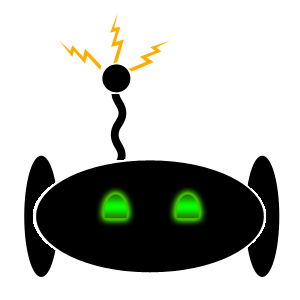
\includegraphics{logotyp.png}}
  	\end{picture}}
	
  \fancyhead[C]{\small{Mapmaster2001}}
  \fancyhead[R]{\small \today}
  \fancyfoot[L]{\small{TSEA56 \\ LIPS Kappa}}
  \fancyfoot[C]{\small{\thepage}}
  \fancyfoot[R]{\small{Projektgrupp 8 \\ mapmaster2001@cyd.liu.se}}

  %-----------------------------------------------------------------

%-------------------------------------------------------------------
%Första sidan

\begin{document}
	\pagestyle{fancy}
\pagenumbering{roman}
	\vspace*{\fill}
		\begingroup
			\begin{center}
				\huge{\textbf{Teknisk dokumentation}}
				\\
				\vspace{5pt}
				\normalsize
				Kandidatprojekt Y - Grupp 8 - VT2014
				\\
				Version 1.0
				\end{center}
		\endgroup
	\vspace*{\fill}
	
	\begin{center} %Börjar centrering 
		Status
		\\
		\vspace{3pt} %Whitespace 3 pts
	    \begin{tabular}{| p{3cm} | p{3cm} | p{3cm} |} %tabell, 4 horizontella |, 3 cm emellan dem.
	    \hline %översta horizontella linjen.
	    Granskad & NE,TG,HFE & \today \\ \hline % & -tecken för att "gå till nästa ruta" 
		Godkänd & - & - \\ \hline % avslutas med \\ och \hline.

	    \end{tabular}
	\end{center}
	\vspace{2cm}
	\newpage
%-----------------------------------------------------------------
%Projektidentitet
	
	\vspace*{\fill}
		\begingroup
			\begin{center}
				\LARGE{\textbf{PROJEKTIDENTITET}}
				\\
				\footnotesize
				Grupp 8, 2014/VT, MapMaster2001
				\\
				Linköpings tekniska högskola, ISY
				\\
				\vspace{1cm}
	  \begin{tabular}{| p{3cm} | p{4.3cm} | p{2.4cm} | p{3.8cm} |}
	    \hline
		\textbf{Namn} & \textbf{Ansvar} & \textbf{Telefon} & \textbf{E-post} \\ \hline
	    Jens Edhammer & Dokumentanvsvarig (DOK) & 076-030 67 80 & jened502@student.liu.se \\ \hline
		Erik Ekelund & Designansvarig (DES) & 073-682 43 06 & eriek984@student.liu.se \\ \hline
		David Habrman &  & 976-017 71 15 & davha227@student.liu.se \\ \hline 
		Tobias Grundström & Testansvarig (TES) & 073-830 44 45 & tobgr602@student.liu.se \\ \hline 
		Hans-Filip Elo &   & 073-385 22 32 & hanel742@student.liu.se \\ \hline 
		Niklas Ericson & Projektledare (PL) & 073-052 27 05 & niker917@student.liu.se \\ \hline
	    \end{tabular}
		
		\vspace{1cm}
		\textbf{E-postlista för hela gruppen:} mapmaster2001@cyd.liu.se
		\\[0.5cm]
		
		\textbf{Kund}: Mattias Krysander, Linköpings Universitet, 581 83  LINKÖPING, \\
		013-28 21 98, matkr@isy.liu.se \\
		\textbf{Kontaktperson hos kund}: Mattias Krysander, 013-28 21 98,matkr@isy.liu.se 
		\\
		\textbf{Kursansvarig}: Tomas Svensson, 3B:528,013 28 21 59,tomass@isy.liu.se
		\\[0.5cm]
		\textbf{Handledare}: Peter Johansson, 013-28 1345 peter.a.johansson@liu.se

				\end{center}
		\endgroup
	\vspace*{\fill}
\newpage

%-----------------------------------------------------------------
%Innehållsföreteckning

\addto\captionsswedish{\renewcommand{\contentsname}{Innehållsförteckning}}

\tableofcontents
\newpage
\listoffigures
\thispagestyle{fancy}
\newpage

\pagenumbering{arabic}

%-----------------------------------------------------------------
%Översikt

\section{Inledning} 
MapMaster2001 är en robot vars uppgift är att underlätta för nödpersonal vid uppdrag i gasfyllda eller rökfyllda lokaler. MapMaster2001 kan skickas in i brandhärjat rum, alternativt ett rum med en gasläcka, innan undsättningspersonal skickas in. 

MapMaster2001 kartlägger sin omgivning och skickar sedan information om denna till en persondator som ritar ut en karta på en skärm. MapMaster2001 hittar eldhärden och markerar denna på kartan så att undsättningspersonal enkelt kan släcka elden. 

\subsection{Syfte och Mål}
Robotens syfte är att kartlägga ett rum och finna en fiktiv eldhärd så snabbt som möjligt. 

\newpage
\section{Produkt}

\begin{figure}[htp] %Placera här om det finns plats, annars så snart som möjligt, på toppen av en sida.
  \begin{center}
  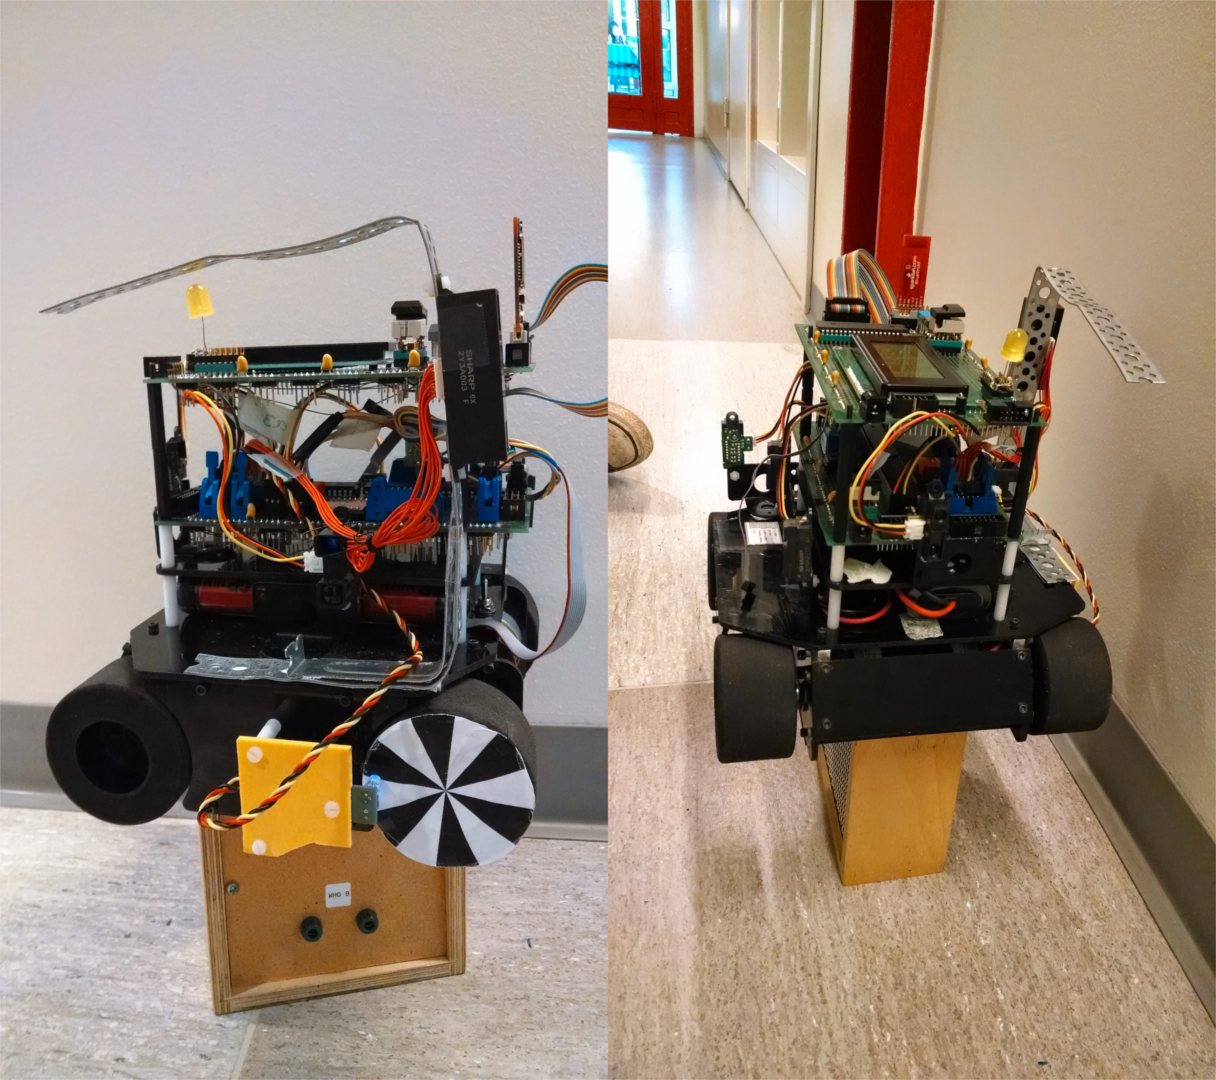
\includegraphics[keepaspectratio=true,,width=0.5\linewidth]{../Kappa/robot.png}  %skala och filnamn. 
  \end{center}
  \caption{MapMaster2001} %figurtext.
  \label{fig:robot}
\end{figure}

Det här är MapMaster2001. En kartritande robot med bred funktionalitet. MapMaster2001 kan bland annat: 

\begin{itemize}
  \item Kartlägga slutna rum
  \item Reglera längs väggar
  \item Läsa av sin omgivning med 6 avståndssensorer
  \item Mäta sin färdväg med en reflexsensor
  \item Indikera autonomt/manuellt läge med en lysdiod
  \item Styras via Bluetooth med hjälp av en persondatormjukvara med ett modernt GUI
  \item Spara sensordata på persondator och plotta denna via inbyggd grafritningsfunktion
\end{itemize}

All mjukvara tillhörande MapMaster2001 samt dokument finns att hitta på GitHub\footnote{https://github.com/hansfilipelo/MapMaster2001}

\newpage
\section{Teori}


\subsection{Kartläggning}


\begin{figure}[htp] %Placera här om det finns plats, annars så snart som möjligt, på toppen av en sida.
  \begin{center}
  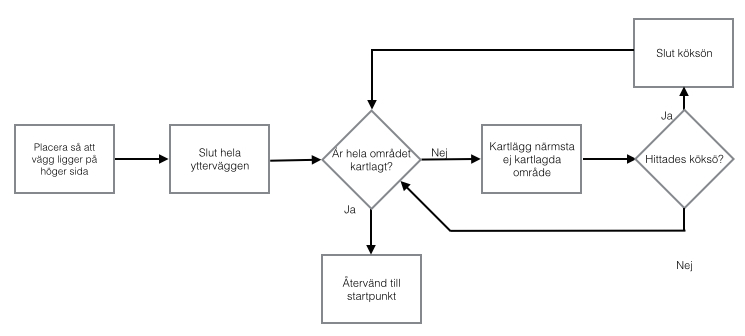
\includegraphics[keepaspectratio=true,scale=0.5]{bilder/Flode_kartritning.jpg}  %skala och filnamn. 
  \end{center}
  \caption{Flödesschema kartläggning} %figurtext.
  \label{fig:mapFlow} %glöm inte att uppdatera era labels
\end{figure}

Djupare teori kring kartläggning och positionering finns i Appendix


%-----------------------------------------------------------------
%Systemet
\newpage
\section{System}

\begin{figure}[htp] %Placera här om det finns plats, annars så snart som möjligt, på toppen av en sida.
  \begin{center}
  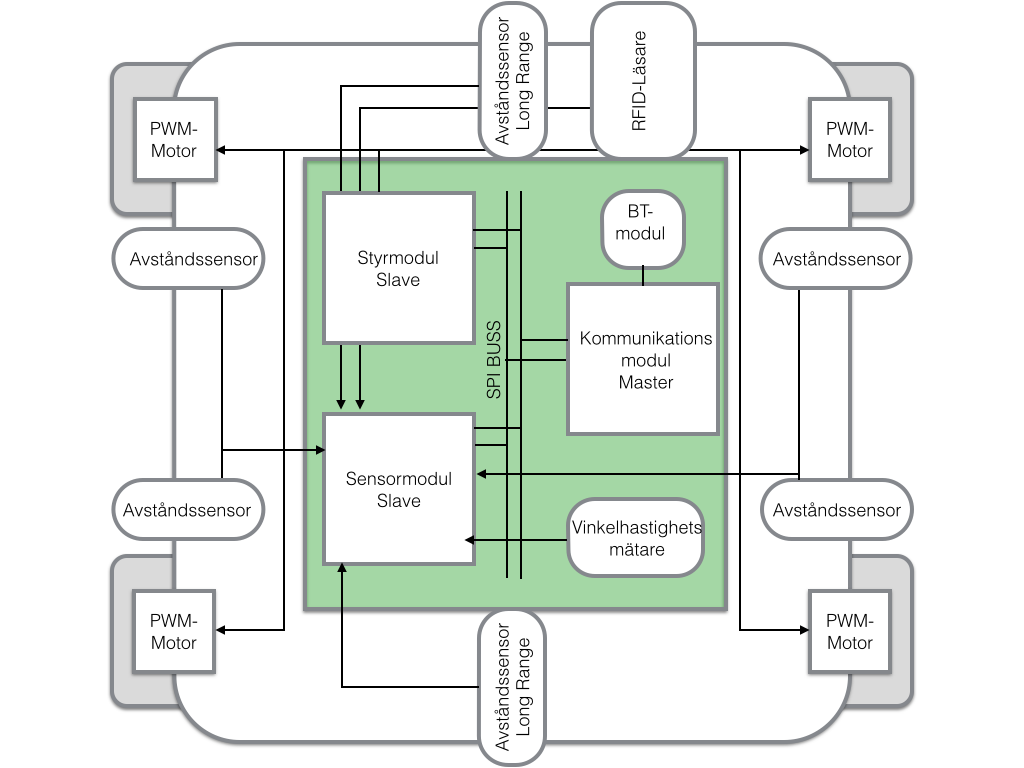
\includegraphics[keepaspectratio=true,width=\linewidth]{bilder/overview}  %skala och filnamn. 
  \end{center}
  \caption{Översiktsbild av systemet} %figurtext.
  \label{fig:overview}
\end{figure}

Roboten består tre delsystem. En kommunikationsmodul, en sensormodul och en styrmodul. Utöver dessa tre moduler finns en buss mellan den, ett chassi samt en tillhörande mjukvara för persondator. Sensormodulen hanterar analoga sensorsignaler och omvandlar dessa till användbart mätdata som skickas vidare till kommunikationsmodulen och styrmodulen. 
Kommunikationsenheten agerar buss-master och sköter all kommunikation mellan de andra enheterna. Kommunikationsmodulen sköter även kommunikationen mellan PC och roboten via en bluetoothadapter. Styrenheten sköter robotens fyra drivande motorer, kartläggning och positionsskattning samt tar beslut om körriktning vid autonom operation. 
De tre delsystemen kommunicerar via en SPI-buss och är byggda runt processorerna ATMEL Atmega 1284p med 16KByte SRAM. 

Chassit har fyra PWM-motorer, placerade längst fram och längst bak på sidorna av chassit. Motorerna är monterade i chassit, vilket betyder att rotation utförs genom att en rotationshastighetsdifferens införs mellan motorparen. Rotationer görs alltid med 90 graders svängar som utförs med hjälp av gyrot som är placerat på sensormodulen. 

Sensorerna som tillhör sensormodulen, förutom robotens RFID-läsare,är placerade på ett sådant sätt att sensorer interfererar minimalt med varandra. En långdistanssensorer av typ GP\-2Y\-3A\-00\-3K\-0F är placerad bak på roboten och används för positionering. På höger sida av roboten har 2 stycken kortdistanssensorer placerats för att ge indata till PD-regleringen. På vänster sida sitter en medeldistanssensor som kommer användas för att upptäcka sidokorridorer och öppna ytor.
Under roboten sitter en RFID-läsare för upptäcka RFIDmarkerade brandhärder.

\subsection{Kommunikation via buss}
En buss som kommunicerar över protokollet SPI sköter kommunikationen mellan robotens tre delsystem. SPI-protokollet är ett fullt-duplext kommunikationsprotokoll som fungerar genom att byta 8 lokala bitar med 8 bitar från modulen den kommunicerar med. 

I mjukvarulagret av bussen användes ett egenimplementerat protokoll som används för både transmissioner över Bluetooth och SPI. Protokollet är konstruerat så att den första byten definierar alltid längden på meddelandet. Nästföljande 2 bytes definierar kommandotyp och argument till den typen. Efter de 3 första bytes följer godtyckligt lång datamängd se figur 3. 

Specificerat bussprotokoll är enbart halv-duplex, d v s man kan enbart skicka data i en riktning åt gången, hela kapaciteten hos SPI utnyttjas alltså inte. 

\begin{figure}[htp] %Placera här om det finns plats, annars så snart som möjligt, på toppen av en sida.
  \begin{center}
  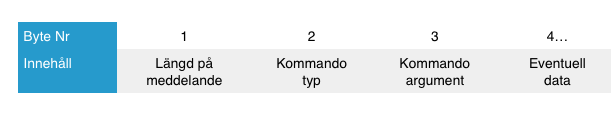
\includegraphics[keepaspectratio=true,scale=0.6]{bilder/Bussprotokoll.png}  %skala och filnamn. 
  \end{center}
  \caption{Översiktsbild av kommunikationsprotokollet} %figurtext.
  \label{fig:bussprotocol}
\end{figure}

Bussens tillgängliga kommandon är:

\begin{tabular}{| p{0.25\textwidth} | p{0.15\textwidth} | p{0.075\textwidth} | p{0.075\textwidth} | p{0.35\textwidth} |}
	\hline
	\rowcolor{listinggray}
	\textbf{Funktion} & \textbf{Datalängd} & \textbf{Kodord} & \textbf{ev argument} & \textbf{datastruktur} \\ \hline
	Rotera vänster & 3 & r & 0 & Hastighet (0-100) \\ \hline
	Rotera höger & 3 & r & 1 & Hastighet (0-100) \\ \hline
	halt & 1 & h & DNC & DNC \\ \hline
	Kör framåt & 3 & f & DNC & Hastighet (0-100) \\ \hline
	Kör bakåt & 3 & b & DNC & Hastighet (0-100) \\ \hline
	Aktivera autonomt läge & 1 & a & DNC & DNC \\ \hline
	Aktivera manuellt läge & 1 & q & DNC & DNC \\ \hline
	Säg åt styrmodul att skicka karta & 1 & F & DNC & DNC \\ \hline
	Sätt variabler för reglering & 11 & P & 0 & Kp(10-tal, 1-tal, 10-del, 100-del), Kd(10-tal, 1-tal, 10-del, 100-del), Referensavstånd \\ \hline
	Sensordata & 26 & S & DNC & Sensor0(100-tal, 10-tal, 1-tal), Sensor2... , Sensor6(100-tal, 10-tal, 1-tal) \\ \hline
	Kalibrera gyro & 2 & g & 0 & DNC \\ \hline
	Börja mäta med gryo & 2 & g & 1 & DNC \\ \hline
	Svängt 90 grader & 1 & G & DNC & DNC \\ \hline
	RFID detekterad & 1 & R & DNC & DNC \\ \hline
	Tillåt RFID-avläsning & 1 & r & DNC & DNC \\ \hline
	En rad av kartan & 19 & M & Radnr & Chars (u, c, e eller f) \\ \hline
	Konfirmering av mottagen kartrad & 2 & m & Radnr & DNC \\ \hline
\end{tabular}
~\\
Där DNC står för ''Do not care''.

% ----------------------------- Kommunikationsmodul ------------------------------
% --------------------------------------------------------------------------------


\section{Kommunikationsmodul}
Modulen hanterar kommunikation mellan robotens olika delkomponenter samt med persondatorn via Bluetooth. Kommunikationsmodulen som syns i figur 3, kommer att agera master på robotens interna buss. Vid kommunikation mellan övriga moduler, dvs. sensor- och styrmodulen, kommer denna gå via kommunikationsmodulen. Kommunikationsmodulen levererar sensordata och manuella styrkommandon mellan roboten och PC-mjukvaran.

\begin{figure}[htp] %Placera här om det finns plats, annars så snart som möjligt, på toppen av en sida.
  \begin{center}
  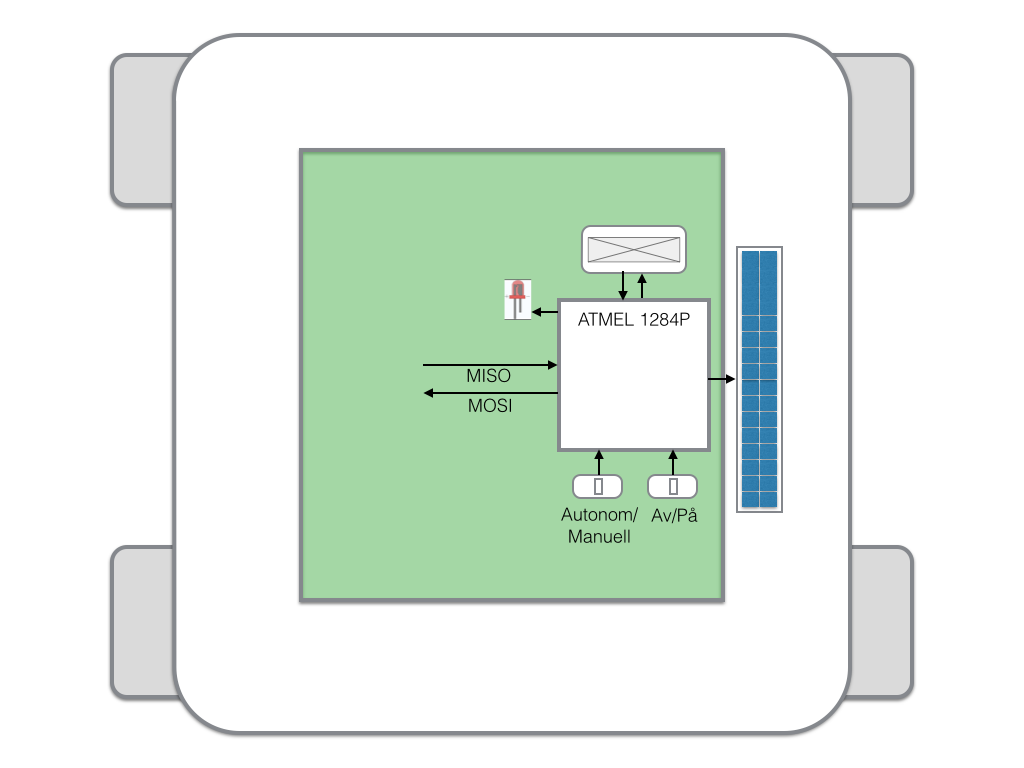
\includegraphics[keepaspectratio=true,width=\linewidth]{bilder/kom_overview.png}  %skala och filnamn. 
  \end{center}
  \caption{Översiktsbild av kommunikationsdelen av systemet} %figurtext.
  \label{fig:overviewKom}
\end{figure}
\newpage
\subsection{Kommunikationsfall}
Ett par exempel på kom\-mun\-ikations\-fall.

Kommunikationsmodulen skickar data mellan de olika enheterna. Ett par olika kommunikationsfall demonstreras i flödesdiagramm i Appendix B.

Fall 1: Kommunikationsmodulen skickar manuella styrkommandon till styrmodulen, se figur~\ref{fig:case1flow}.

Fall 2: Sensormodulen signalerar att ny sensordata är redo, se  figur~\ref{fig:case2flow}.

Fall 3: Kartdata skickas från kommunikationsmodulen till PC, se figur~\ref{fig:case3flow}. 
 
\subsection{Komponenter}
\begin{itemize}
  \item AVR processor av typen ATMega1284
  \item Bluetoothsdongel, Firefly, BlueSmirf Gold
  \item LCD-Display
  \item Två stycken knappar
  \item Kristalloscillator EXO-3, 14.745 MHz
  \item Lysdiod
  \item Bandkabel
\end{itemize}

\subsection{Buss}
Mellan processorerna används SPI som bussprotokoll. Kommunikationsmodulen agerar master medan styr- och sensormodul agerar slaves. Kommunikation kommer alltid att initieras av master och om slave vill skicka data, genererar de ett avbrott på master som talar om att de har data som är redo att skickas. 

Mellan processorerna används SPI som bussprotokoll. Kommunikationsmodulen agerar master medan styr- och sensormodul agerar slave. Kommunikation kommer alltid att initieras av master och om slave vill skicka data, genererar de ett avbrott på master som talar om att de har data som är redo att skickas. Bussen använder följande kopplingar för bussen:
\begin{itemize}
	\item MISO - Master Input Slave Output, data till master
	\item MOSI - Master Output Slave Input, data till slave
	\item SLAVEINT0 - Avbrott från slave 0
	\item SLAVEINT1 - Avbrott från slave 1 
	\item SLAVESELECT0 - Väljer denna processor som aktiv slav
	\item SLAVESELECT1 - Väljer denna processor som aktiv slav
	\item SCK - Serial Clock, klocka från master
\end{itemize}

\subsubsection{Slav-modulers mottagning}
När vår master-modul initierar SPI-kommunikationen med en slave dras SlaveSelect-signalen för den givna processorn låg för att generera ett SPI-avbrott på sagda slave. När slave har tagit emot det antal bytes som specificeras av första byten i paketet genereras ett internt avbrott med hjälp av PCint16. I detta nya avbrott hanteras datan från transmissionen. En övergripande struktur angående mottagningen av SPI-trafik kan ses i flödesdiagrammet i figur~\ref{fig:spislave}

\begin{figure}[htp] %Placera här om det finns plats, annars så snart som möjligt, på toppen av en sida.
  \begin{center}
  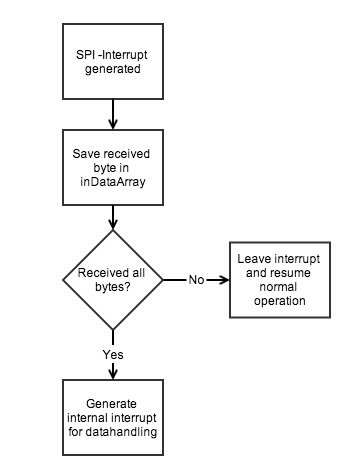
\includegraphics[keepaspectratio=true,width=0.4\textwidth]{bilder/spislaverec.jpg}  %skala och filnamn. 
  \end{center}
  \caption{Översiktsbild av mottagning för en SPI-slav} %figurtext.
  \label{fig:spislave}
\end{figure}

\subsubsection{Busstrafik}
På bussen kommer ett antal olika typer av kommandon att skickas. Dessa förklaras i paragraferna nedan. 
Tyngre och snabbt på varandra följande transmissioner kan leda till låsningar av bussen i form av att till exempel sensordata slutar levereras till Bluetoothmodulen eller att ett kommando missas. Därför hanteras de tyngsta transmissionerna med en konfirmationsstruktur.
De tyngsta kommandona utförs endast på ickekritiska tillfällen i respektive slavmodul.

\paragraph{Styrkommandon från PC}
~\\
När styrkommandona skickas från PC, kommer kommunikationsmodulen skicka datan vidare till styrmodulen som utför kommandot.
\paragraph{Konverterat sensordata}
~\\
Sensordata kommer att behandlas i sensormodulen och därefter kommer modulen att skicka ett avbrott till master om att data finns tillgängligt. Mastern svarar och startar bussöverföringen.
\paragraph{Kartabstraktion så styrenheten kan välja färdväg}
~\\
Kartabstraktionen och robotens position kommer att uppdateras allt eftersom ny sensordata kommer in. Efter att ny sensordata har mottagits av master skickar mastern ut sensordata till styrenheten.
\paragraph{Kommandon för inställning av reglerparametrar.}
~\\
Kommandon mottags via blåtand från PC på mastern, som skickar detta vidare till styrenheten. 
\paragraph{RFID aktivering och bekräftelse}
~\\
Kommandot skickas från styrmodulen via mastern som speglar ner kommandot till sensormodulen. Sensormodulen startar då RFID-läsning och skickar bekräftelse till styrmodulen när RFID-kortet är detekterat.  

\paragraph{Gyro aktivering och bekräftelse}
~\\
Kommandot skickas från styrmodulen via mastern som speglar ner kommandot till sensormodulen. Sensormodulen startar då Gyro-omvandling och skickar bekräftelse till styrmodulen när roboten har roterat 90 grader. 

\paragraph{Hjulsensor aktivering och bekräftelse}
~\\
Kommandot skickas från styrmodulen via mastern som speglar ner kommandot till sensormodulen. Sensormodulen startar då en hjulsensormätning och skickar bekräftelse till styrmodulen när roboten har färdats 40 cm. 

\subsection{LCD-Display}
Sensordata och annan information från roboten visas på en alfanumerisk-display, närmare bestämt  LCD JM162A. Displayen kommer användas för att visa sensordata samt eventuella parametrar för debugging under testfasen.
Displayen kommer anslutas till processorn enligt kretschemat i appendix A. 
Vid varje uppstart kommer initiering av LCD-display göras och då följa nedanstående flödesschema. Varje steg startas med att processorn skickar ett kommando till ingångarna på LCD-displayen. Kommandon finns specificerade i databladet\footnote{https://docs.isy.liu.se/twiki/pub/VanHeden/DataSheets/jm162a.pdf}. LCD-displayen sitter på mastermodulen och för att inte låsa mastermodulen under tiden då datan skrivs ut på diaplyen har ett buffersystem implementerats. Buffersystemet gör så att mainprogrammet i mastern inte låser när data skrivs till displayen. Buffern håller koll på vilken rad och kolumn som för tillfället ska skrivas ut och kan därför avsluta skrivningen direkt efter att ingen eller en karaktär är utskriven på displayen. Därefter kan mastern återgå till mainloopen för att hantera inkommande eller mottagande data. Genom att hantera skrivningar på detta vis undviker vi att låsa kommunikationsmodulen vid de tidskrävande LCD-skrivningarna.

\subsubsection{Uppstart}
	
Vid uppstart av systemet kommer LCD-displayen att initieras enligt flödes\-schemat~\ref{fig:flowlcdstart}

\begin{itemize}
  \item Power ON - sätter på strömförsörjningen
  \item Function set - Sätter överförsdatalängden till 8 bitar och displayläget till 2-rader.
  \item Display ON - slår på displayen och slår på markören. 
  \item Entry mode set - sätter markörens riktning vid skrivning
  \item End - Slut på initieringen
\end{itemize}

\begin{figure}[htp]
	  \begin{center}
	  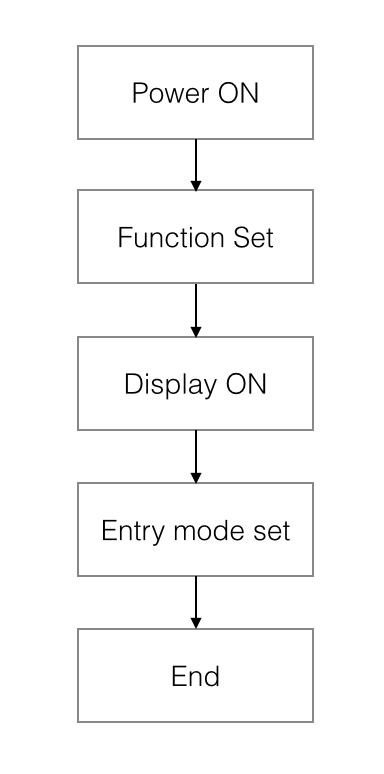
\includegraphics[keepaspectratio=true,width=0.4\linewidth]{bilder/startup}  %skala och filnamn. 
	  \end{center}
	  \caption{Uppstart av LCD-display} %figurtext.
	  \label{fig:flowlcdstart}
	\end{figure}

\newpage


\subsubsection{Skrivning}

Skrivning till LCD-displayen kommer ske enligt flödesschemat~\ref{fig:flowlcdwrite}
\begin{itemize}
  \item Start write procedure - Startar skrivning till LCD-displayen
  \item Clear - Rensar hela displayen
  \item Set DDRAM - gör DDRAMet tillgängligt
  \item Write data to RAM - Skrivning av data in till RAM ifrån DDRAM
\end{itemize}

\begin{figure}[htp] %Placera här om det finns plats, annars så snart som möjligt, på toppen av en sida.
  \begin{center}
  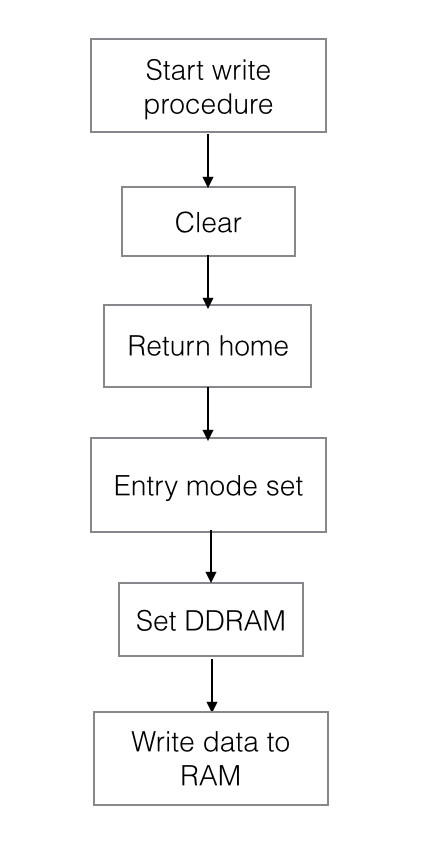
\includegraphics[keepaspectratio=true,width=0.5\linewidth]{bilder/write}  %skala och filnamn. 
  \end{center}
  \caption{Skrivning till LCD-display} %figurtext.
  \label{fig:flowlcdwrite}
\end{figure}

\subsection{Bluetooth}
Bluetoothkommunikationen kommer att utföras av ett Firefly-Bluesmirf gold (FBG) modem som parkopplas mot en persondator.
FBG kommer att skicka information till persondator via protokollet RS232 enligt vad som är angivet på Vanheden. 
Se schema i appendixet Scheman för anslutning av TxD och RxD, vilka sköter sändning och mottagning av data.
När vi skickar data till processorn så är detta avbrottshanterat. I avbrottet utnyttjas en databuffer vid namn inDataArray som sedan kopieras till bufferten pcHandle i datahanteringen av Bluetooth. Även Bluetooth datahanteras utanför avbrotten precis som SPI-kommunikationen.

\subsubsection{Skickning av kartan}
För att undvika problem vid mottagning av kartan på PC sidan skickas en rad i taget med hjälp av en timer. Main-loopen på kommunikationsmodulen kollar en gång per main-loop om det är okej att skicka en rad. När timern genererar ett avbrott sätts en flagga att ytterligare en rad är redo att skicka. När samtliga rader har skickats över sätts flaggan som avgör om kartrader ska skickas över till false. 

\subsection{Switchar}
En switch ska styra om roboten exekverar programkod för autonom styrning eller manuell styrning. Denna switch kan även byta läge via ett virtuellt kommando från PC. Ett avbrott signalerar till processorn att den ska byta programkod, avbrottet ligger på pin16 (INT0) se appendix A. 
Av/På-knappen styr strömförsörjningen till samtliga moduler. 

% ----------------------------- Styrmodul --------------------------------------
% --------------------------------------------------------------------------------

\newpage
\section{Styrmodul}
Styrmodulens (slave) huvudkomponent kommer att bestå av en AVR-processor, Atmel ATmega1284p som får instruktioner från kommunikationsmodulen (master) via bussen. Processorn kommunicerar även med drivkretsen på chassit. Chassit är av typen Terminator som drivs av en NiMH- eller NiCd-ackumulator på 7.2V. Det har även fyra stycken växlade DC-motorer som är kopplade till varsitt drivhjul. 

\begin{figure}[htp] %Placera här om det finns plats, annars så snart som möjligt, på toppen av en sida.
  \begin{center}
  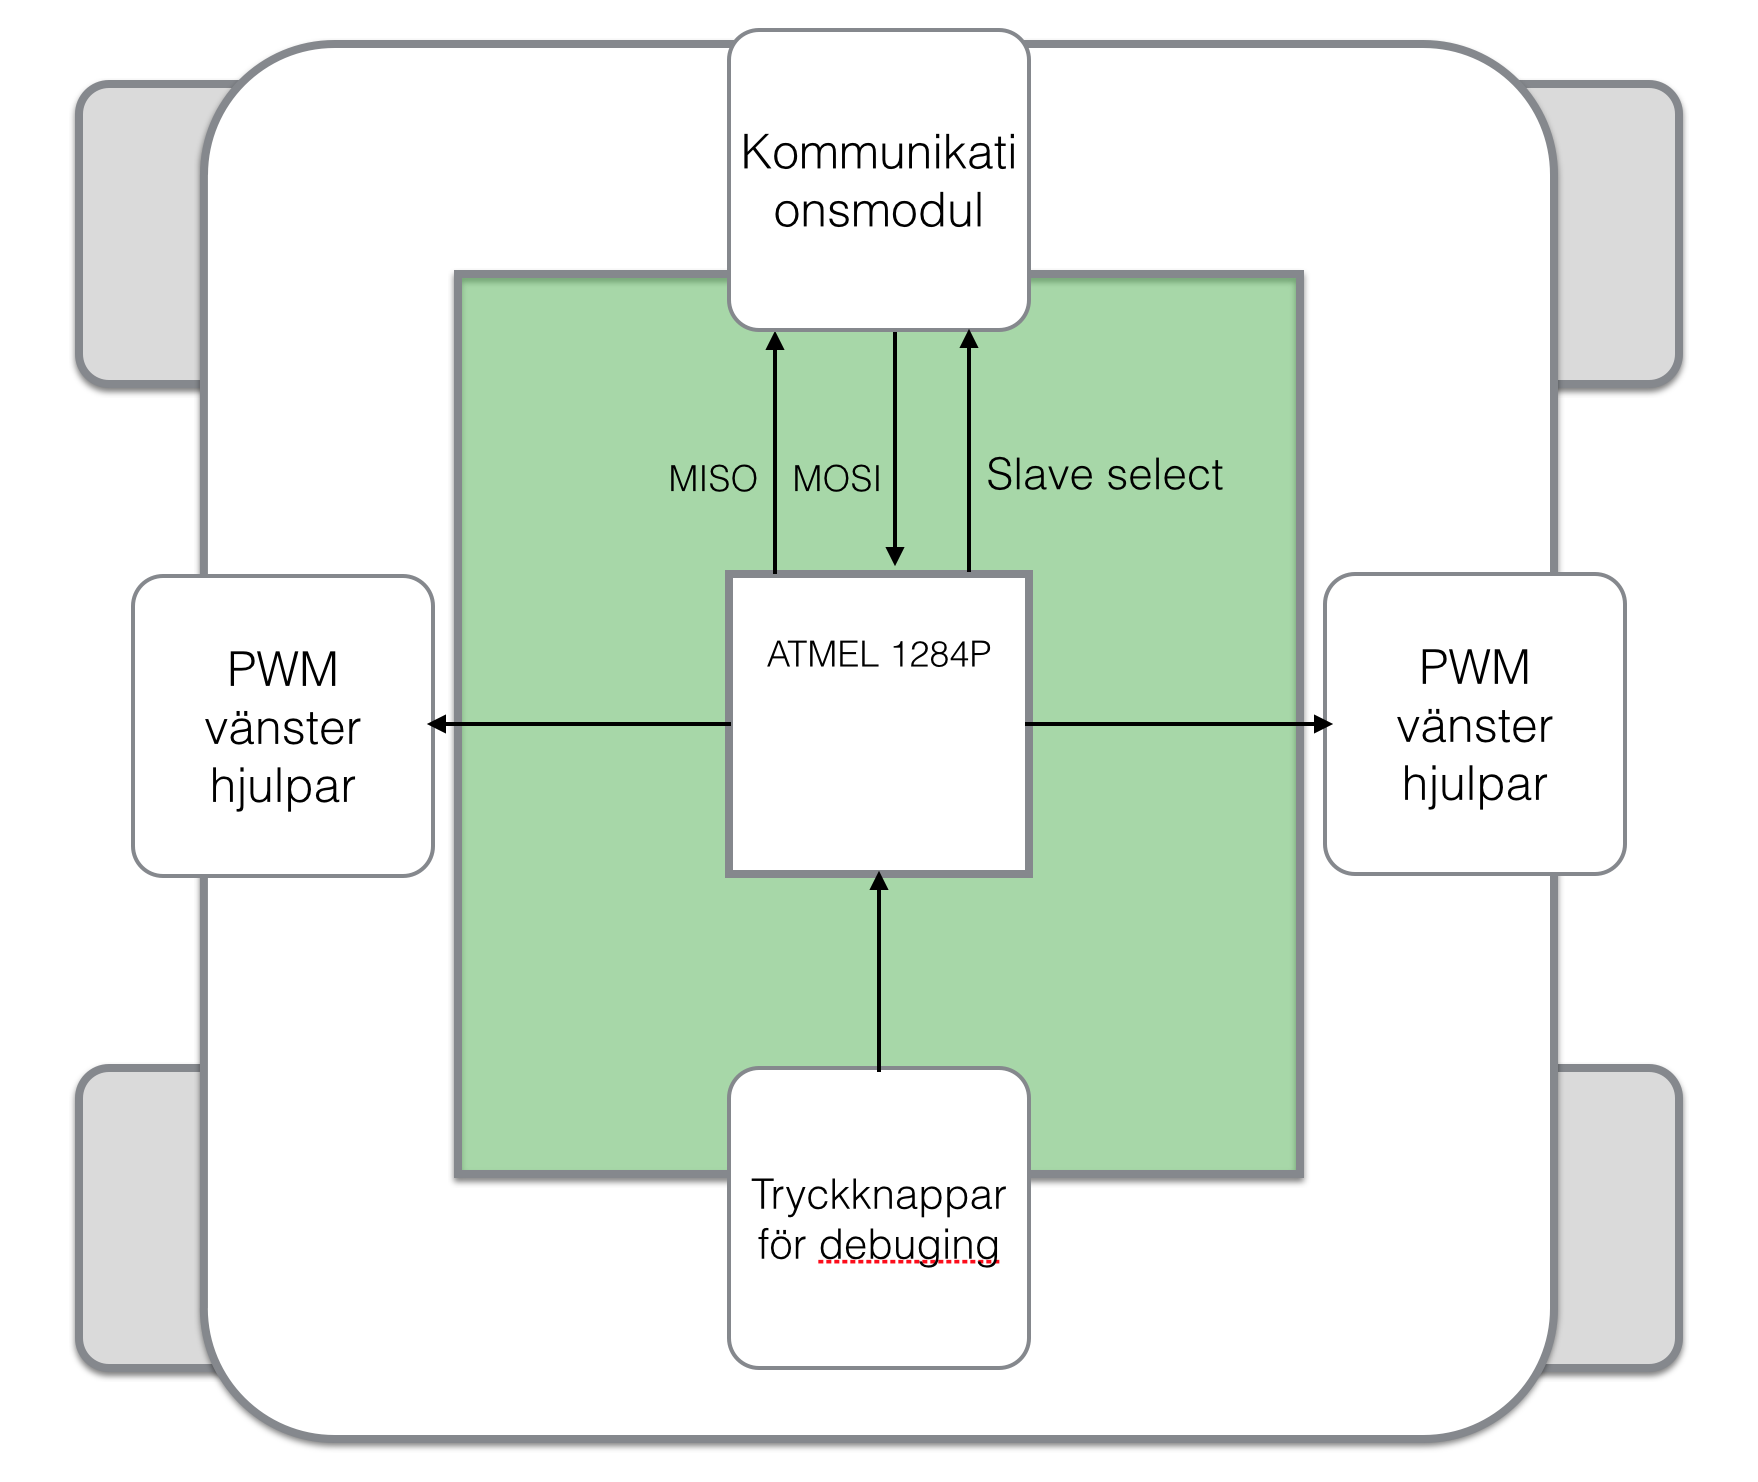
\includegraphics[keepaspectratio=true,width=0.5\linewidth]{bilder/styrmodul}  %skala och filnamn. 
  \end{center}
  \caption{Översikt styrmodul} %figurtext.
  \label{fig:styr} %glöm inte att uppdatera era labels
\end{figure}
\newpage

% ----------- Komponenter ------------------

\subsection{Komponenter}
\begin{itemize}
	\item Chassi
	\item Systemchip - Atmel ATmega1284p (1)
	\item Batteri, 7.2 V
	\item Resetknapp
\end{itemize}
\subsection{Signaler}
Motorerna kommer att styras parvis med två signaler per sida:
\begin{itemize}
	\item DIRL - Styr den vänstra motorns rotationsriktning
	\item DIRR - Styr den högra motorns rotationsriktning
	\item PWML - Pulsbreddmodulerad signal som styr den vänstra motorns hastighet
	\item PWMR - Pulsbreddmodulerad signal som styr den högra motorns hastighet.
\end{itemize}
~\\
Dessa kopplas direkt från processorn till chassits drivkrets enligt bild.
Styrmodulen kommer att vara ansluten till bussen med hjälp av MISO- och MOSI-pinnarna.

\begin{itemize}
	\item MISO - Master Input Slave Output, data skickas till master
	\item MOSI - Master Output Slave Input, data skickas till slave
	\item MASTERINT - Skickar avbrott till master
	\item SLAVESELECT - Väljer denna processor som aktiv slav
	\item SCK - Serial Clock, klocka från master
\end{itemize}
~\\
Utöver detta kommer en tryckknapp anslutas till RESET för att förhindra att felaktig programmering av processorn. 

För fullständigt kopplingsschema - se Appendix. 

\newpage
% ------------------- Styrning och kartläggning -----------------------

\subsubsection{Kartabstraktion}
Kartan abstraheras som en matris där objekt sparas, detta löses i form av en arrays med dimensionerna 32x17.
Tillgängliga undertyper är:

\begin{itemize}
\item{EmptySection}
\item{UnexploredSection}
\item{Robot}
\item{Closed}
\item{Fire}
\end{itemize}

Robot är en egen klass med polymorfiskt arv från mapSection.

\paragraph{EmptySection} 
~\\
EmptySection representeras av en tom sektion av kartan. 

\paragraph{UnexploredSection} 
~\\
UnexploredSection kommer att representera en outforskad sektion av kartan. 

\paragraph{Robot} 
~\\
Robot kommer att representera robotens position på kartan. 

\paragraph{Closed} 
~\\
Om en sektion är stängd sätts den till closed.

\paragraph{Fire} 
~\\
Fire kommer att representera plats där det finns eldhärd, dvs. en RFID-tagg. 
\newpage

% ---------------- Styrning o kartl --------------

\subsection{Styrning och kartläggning}
Det har implementeras två olika avsökningsalgoritmer. Dessa kan aktiveras beroende på vilket uppdrag roboten ska utföra. Algoritmerna kommer att skrivas med hjälp av C++ och köras från processorns interna minne. 

\subsubsection{Kartläggninsalgoritm}

Kartläggningsalgoritmen utformas så att roboten börjar med att placera sig så att en vägg går att finna på höger sida. Roboten kommer sedan följa väggen till dess att den kan rita upp ett slutet område att arbeta utifrån. Nästa steg blir att kartlägga områden som ännu ej är kartlagda. Om en köksö upptäcks kommer roboten se till att rita upp hela köksön innan den går vidare. På detta sätt fortsätter algoritmen till dess att alla delar av rummet är kartlagda. 

\begin{figure}[htp] %Placera här om det finns plats, annars så snart som möjligt, på toppen av en sida.
  \begin{center}
  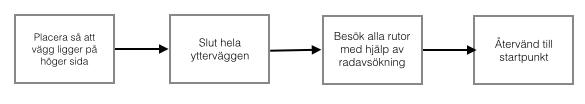
\includegraphics[keepaspectratio=true,width=0.8\linewidth]{bilder/flode_brandhard.jpg}  %skala och filnamn. 
  \end{center}
  \caption{Flödesschema kartläggningsalgoritm} %figurtext.
  \label{fig:map} %glöm inte att uppdatera era labels
\end{figure}

\paragraph{Stänging och slutning av bana}
När roboten har åkt längs högerväggen och återvänder till startkoordinaterna samt har färdriktningen höger i kartabstraktionen anses kartan vara sluten. När kartan är sluten anses fortfarande objekt utanför inramningen att vara outforskade. Då dessa är omöjliga att besöka startas ett anrop till samtliga objekt längs y-axeln på koordinaterna x = 0 och x = 31. Funktionen ber objektet att bli av typen closed om den inte redan är det. Är objektet closed avslutas funktionen där, annars ber den alla sina direkta grannar att även de utföra funktionen. Denna funktion stänger alltså alla objekt i ett område avgränsat av andra closed-objekt.

\newpage

\subsubsection{Brandhärdssökning}

Brandhärdssökningen kommer att gå till på liknande sätt som kartläggningsalgoritmen, dock kommer den vara långsammare på grund av att varje ruta i området måste besökas. Efter att området slutits använder roboten sig av radavsökning för att systematiskt besöka alla rutor. Om en RFID-tag upptäcks ska detta noteras.

\begin{figure}[htp] %Placera här om det finns plats, annars så snart som möjligt, på toppen av en sida.
  \begin{center}
  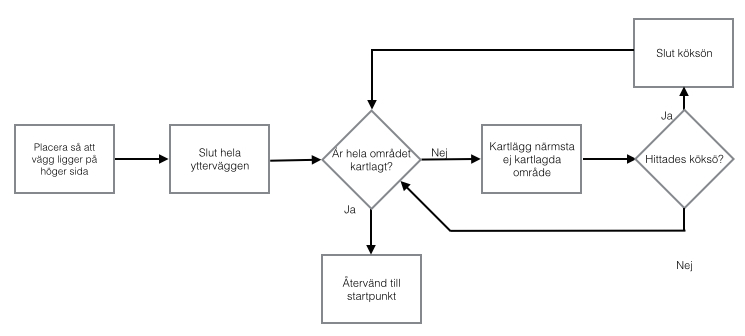
\includegraphics[keepaspectratio=true,width=0.5\linewidth]{bilder/Flode_kartritning.jpg}  %skala och filnamn. 
  \end{center}
  \caption{Flödesschema brandhärdssökning} %figurtext.
  \label{fig:fire} %glöm inte att uppdatera era labels
\end{figure}



% ------------------- Reglering -----------------------

\subsection{Reglering}

Roboten kommer kunna styras dels autonomt men också manuellt via PC-mjukvara. 

\subsubsection{Reglering av styrning}
Styrmodulen kommer att få sensordata skickad till sig från sensormodulen. Detta data kommer att användas till att reglera riktningen då man följer en vägg. Roboten använderts sig av en tvåviktad proportionell reglering 

Den första proportionella delen av regleringen reglerar avståndet från senorerna på robotens högersida jämfört med ett internt referensavstånd. Denna reglering ser till att roboten håller sig inom ett rimligt avstånd till den vägg som följs.
$ e_p = K_{p}*avst\text{\it{å}}ndssensordata $

Där $K_{p}$ är en konstant.

Den andra proportionella reglering försöker minimera differensen mellan båda sensorerna på högersidan. Detta innebär i praktiken att  roboten försöker räta ut sig. Denna typ av reglering medför även en minskad risk att de främre och bakre sensorerna ska ger fel värden genom att slå i en sidovägg.
Den deriverande delen av regleringen ges av differensen mellan den främre avståndssensorn och den bakre: 

$ e_d = K_{D}*(fram - bak) $

Totala felet ges då av: 

$e = e_d + e_p$


% ----------- Kommunikation ------------------

\subsection{Kommunikation}

Styrmodulen kommunicerar med kommunikationsmodulen (master) över SPI-bussen. Bussen kopplas in på dedikerade pinnar för SPI-bussen på ATmega1284p-processorn. Kommunikationsmodulen kommer att agera master på bussen.

De kommandon styrmodulen kommer att kunna hantera beskrivs i tabellen nedan. \newline

\newpage


% ----------------------------- Sensormodul --------------------------------------
% --------------------------------------------------------------------------------

\section{Sensormodul}
Sensormodulens uppgift är att hantera sensordata från robotens 9 sensorer och sända detta vidare till kommunikationsmodulen i ett hanterbart format. Sensormmdulen är byggd kring AVR-processorn ATMEL 1284p. En överblick av systemet visas i figur~\ref{fig:sensoroverview}.

\begin{figure}[htp] %Placera här om det finns plats, annars så snart som möjligt, på toppen av en sida.
  \begin{center}
  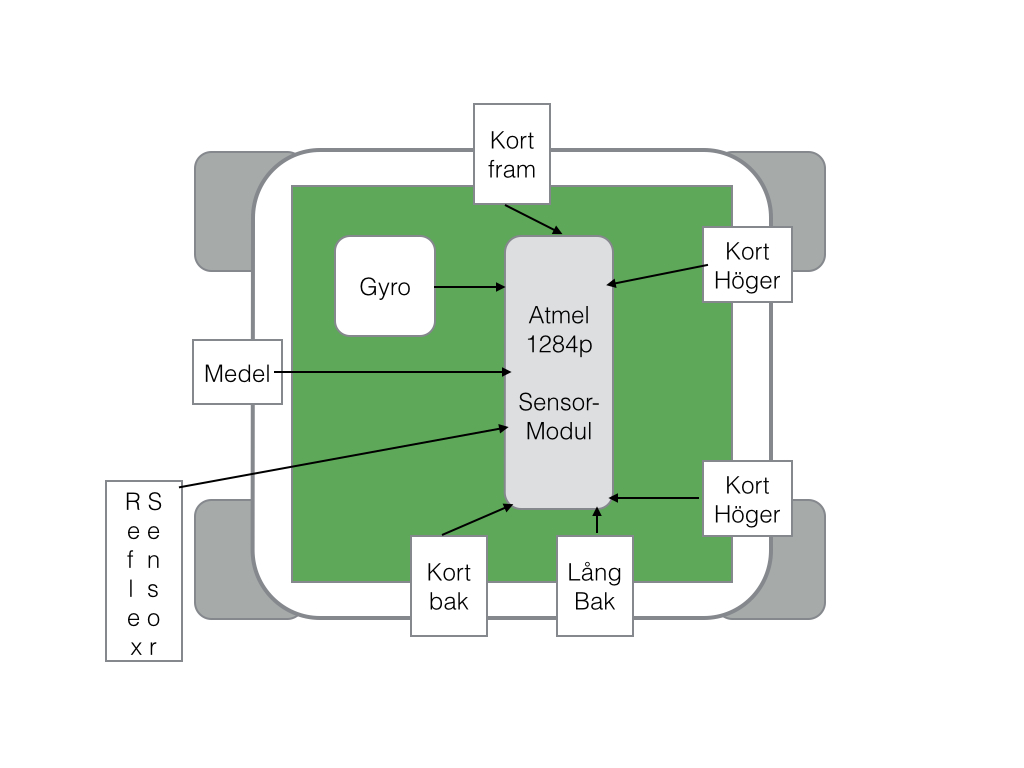
\includegraphics[keepaspectratio=true,width=0.5\linewidth]{bilder/overblicksensor}  %skala och filnamn. 
  \end{center}
  \caption{Överblick av sensormodulen} %figurtext.
  \label{fig:sensoroverview}
\end{figure}

\subsection{Kopplingsschema}

En beskrivande bild av kopplingsschemat finns i appendix A.

\begin{figure}[htp] %Placera här om det finns plats, annars så snart som möjligt, på toppen av en sida.
  \begin{center}
  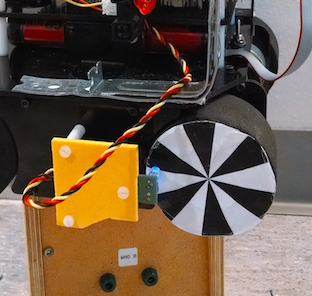
\includegraphics[keepaspectratio=true,width=0.5\textwidth]{../Kappa/reflexsensor.png}  %skala och filnamn. 
  \end{center}
  \caption{Reflexsensor} %figurtext.
  \label{fig:reflex} %glöm inte att uppdatera era labels
\end{figure}

Port A användas som en A/D-omvandlare. PIN 39 kopplas till en reflexsensor, se figur \ref{fig:reflex}, SFH300, PIN 40 kopplas till en avståndssensor för långdistans, GP\-2Y\-3A\-00\-3K\-0F, PIN 35-38 kopplas till avståndssensorer för kortdistans, GP\-2Y\-0A\-21\-YK, 
PIN 34 kopplas till en avståndssensor för mellandistans, GP2Y0A02YK, och PIN 35 kopplas till ett gyro för vinkelhastighetsmätning, ML\-X9\-06\-09. Port B används för busskommunikation. PIN 3 skickar avbrott till master, PIN 5 används till slave select master, PIN 6 tar emot data från bussen, PIN7 skickar data till bussen och till PIN 8 kopplas klockan från master. Till port C PIN 23 kopplas en RFID-läsare, Parallax-Reader. Port D används inte i denna modul. 

PIN 31 och 11 kopplas till jord, PIN 13 kopplas till klocka från master, PIN 12 används inte i denna modul, PIN 9 kopplas till en avstudsad manuell switch, en resetknapp, PIN 32 kopplas till en spänningskälla på 5 V som används som referensspänning, PIN 10 kopplas också den till en spänningskälla på 5 V och PIN 30 kopplas genom ett LP-filter till samma externa spänningskälla.


\subsection{Uppgift}
Sensormodulens uppgift är att A/D-omvandla signaler från robotens avståndssensorer, reflexsensor och gyro för att sedan utnyttja dessa digitala värden för att uppskatta avstånd och tillryggalagd sträcka. Den har också som uppgift att detektera brandhärdar i form av RFID-taggar. I figur~\ref{fig:sensorflow} beskrivs hanteringen av sensordata.

\begin{figure}[htp] %Placera här om det finns plats, annars så snart som möjligt, på toppen av en sida.
  \begin{center}
  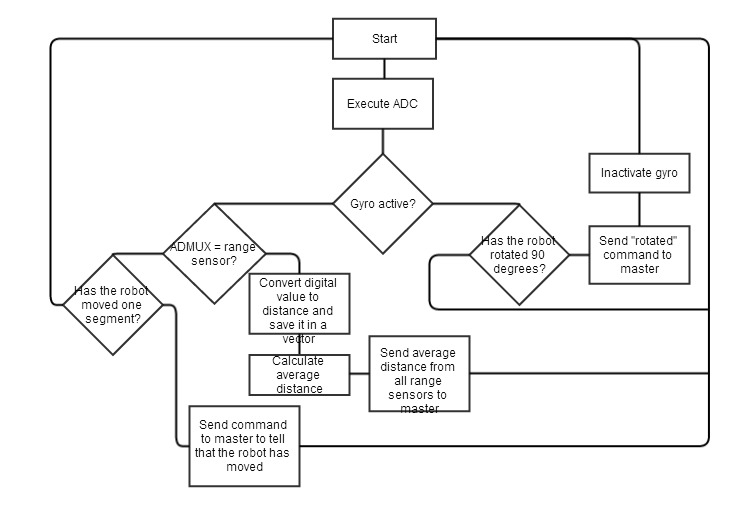
\includegraphics[keepaspectratio=true,width=0.6\linewidth]{bilder/sensorflode}  %skala och filnamn. 
  \end{center}
  \caption{Flödesdiagram för sensorhantering} %figurtext.
  \label{fig:sensorflow}
\end{figure}

\subsection{Komponenter}
\begin{itemize}
	\item Systemchip - Atmel ATmega1284p
	\item RFID-sensor - Par\-all\-ax-Read\-er\
	\item Reflexsensor - SFH300
	\item Avståndssensor för längre avstånd - GP\-2Y3A\-00\-3K\-0F
	\item Avståndssensor för mellan avstånd - GP2Y0A02YK
	\item 4 st avståndssensorer för kortare avstånd - GP\-2Y\-0A\-21\-YK
	\item Vinkelhastighetssensor - MLX\-90\-609
\end{itemize}
~\\

\subsubsection{Systemchip}
Modulens processor är en Atmel ATmega1284p\footnote{\url{http://www.atmel.com/ja/jp/Images/doc8059.pdf}}. Processorn kommer kontinuerligt att hämta data från alla sensorer via processorns inbyggda A/D-omvandlare med tillhörande mux. Denna är programmerbar och kommer att innehålla de program som behövs för att konvertera signalerna till avstånd, tillryggalagd sträcka och detektion av RFID-tagg. Sensormodulen bildar ett medelvärde, beräknat från 25 mätningar, från varje avståndssensor och skickar det kontinuerligt till master, 
kommunikationsmodulen, via en SPI-buss.

\subsubsection{RFID-sensor}
För att kunna detektera RFID-taggen så krävs en RFID-läsare. Vi kommer att använda Par\-all\-ax-Read\-er\footnote{\url{https://docs.isy.liu.se/twiki/pub/VanHeden/DataSheets/rfid-reader-v21.pdf}}. 
SOUT på RFID-sensorn, PIN 3, kopplas till port C, PIN 23, på processon. RFID-läsaren använder sig av serielprotokollet asynkron USART för att skicka data från RFID-korten vidare till CPU:n. Pinne 23 som RFID-läsaren är inkopplad på har stöd för seriell kommunikation och konfigureras för att matcha dataöverföringshastigheten från läsaren.

<<<<<<< Local Changes
Då brus kan ge upphov en falsk RFID-läsning, så kontroller=======
Då brus kan ge upphov en falsk RFID-läsning, så kontrolleras att mottaget data matchar vissa symboler. Vi har valt att leta efter en start byte, 0x0A, som indikerar början på en RFID-taggs unika id. För att ytterligare säkerställla en korrekt läsning görs denna kontroll två gånger innan kommandot för upptäckt brandhärd skickas till master.

\subsubsection{Reflexsensor}
Reflexsensorn, SFH300 som går att läsa om på Vanheden\footnote{\url{https://docs.isy.liu.se/twiki/pub/VanHeden/DataSheets/sfh300.pdf}}, används för att beräkna tillryggalagd sträcka. Sensormodulen skickar ett kommando till styrmodulen då roboten åkt 40 cm, alltså då roboten kommit till ett nytt 40x40-segment. För att beräkna den tillryggalagda sträckan fästs en pappersskiva på ett av robotens hjul. Skivan består av 6 vita och 6 svarta lika stora ''tårtbitar''. Reflexsensorn detekterar varje gång skivan byter färg och på så sätt kan sträckan räknas ut.

\subsubsection{Avståndssensorer}
Roboten kommer att ha sex stycken av\-stånds\-sensorer varav en är för lång\-distans, GP\-2Y3A\-00\-3K\-0F 40-300 cm som går att läsa om på Vanheden\footnote{\url{ https://docs.isy.liu.se/twiki/pub/VanHeden/DataSheets/gp2y3a003k0f.pdf }}, en för mellan\-distans, GP2Y0A02YK 20-150 cm som går att läsa om på Vanheden\footnote{\url{https://docs.isy.liu.se/twiki/pub/VanHeden/DataSheets/gp2y0a02_e.pdf}}, och resterande 4 är för \hyphenation{kort-dist-ans},GP\-2Y\-0A\-21\-YK 10-80 cm som finns på Vanheden\footnote{\url{https://docs.isy.liu.se/twiki/pub/VanHeden/DataSheets/gp2y0a21.pdf}}. Långdistanssensorn placeras fram på roboten och mellandistanssensorn placeras på robotens vänstra sida. Två av kortdistanssensorerna placeras på robotens högra sida, en placeras fram på roboten och den sista placeras på robotens baksida.

PIN 6 på långdistanssensorn och PIN 1 på kortdistanssenorerna och mellandistanssensorn kopplas till port A, PIN 39, PIN 35-38 respektive PIN 34 på processorn. Sensorerna skickar alltså sin data till processorn för A/D-omvandling och tolkning.

GND på sensorerna sätts till jord, Vcc och Vin sätts till hög och PIN 3 på långdistanssensorn sätts till hög.
 
Data från sensorerna behövs för att detektera väggar och skapa en kartabstraktion. Data sensorerna på sidan används för att reglera roboten under färd och sensorerna framtill och baktill används, som nämnts ovan, för att trimma reflexsensorn.

\subsubsection{Vinkelhastighetssensor (gyro)}
För att underlätta beräkningar av körriktningar och hålla koll på hur mycket roboten svängt används en vinkelhastighetssensor eller gyro, MLX\-90\-609 på Vanheden \footnote{\url{https://docs.isy.liu.se/twiki/pub/VanHeden/DataSheets/MLX90609\_datasheet.pdf}}. OUTAR på gyron, PIN 24, kopplas direkt till bussen för att minska brus. Gryot skickar en spänning mellan 0.5 och 4.5 V där 2.5 V motsvarar vinkelhatsighet noll. Sensormodulen börjar mäta på gryot då ett kommando från styrmodulen mottagits. Sensormodulen skickar i sin tur tillbaka ett kommando då roboten svängt 90 grader. Sensormodulen låser sig till endast mätningar på gyroskopet under svängar.

Då roboten endast kommer att använda sig av ortogonala svängar så räcker det med att gyrot används för att mäta ortogonala svängar. Om man adderar vinkelhasigheter med ett jämt tidsintervall så blir summan alltid lika stor vid 90 grader.
Summan som används har tagits fram och kalibrerats med hjälp av tester.

\subsubsection{Övriga komponenter}
Övriga komponenter så som ett batteri på 7.2 V och en resetknapp kommer att användas till denna modul.

\subsection{Övergripande design}
Sensorerna kommer att vara placerade engligt bilden i figur \ref{fig:sensoroverview} .

\section{PCmjukvara}
Det grafiska gränssnittet är skriver i Qt 5.3.0 och är designad i QtCreator och mjukvaran är skriven för att vara kompatibelt med MacOSX.
Qt har eventhantering. Qt kallar dessa events för slots och de kan liknas med avbrott.
\subsection{Bluetooth}
Bluetooth mottagningen på PC fungerar genom att modulen i PC virtualiserar en seriellport som sedan data kan skickas på. För att skapa porten utnyttjas den inbyggda klassen i Qt, QSerialPort. Denna initialiserar Bluetooth kopplingen och sätter inställningar som läs-skriv läge, BaudRate, antal databitar, paritet och stopbitar.
Det är alltid exakt 27 bytes per transmission.

\subsection{Läsning av Bluetooth}
När data kommer till Bluetooth-enheten skickas ett avbrott till mainprogrammet och denna påbörjar mottagning i funktionen HandleReadyRead(). Denna funktion förklaras i flödesdiagrammet figur~\ref{fig:BTpc}

\begin{figure}[htp] %Placera här om det finns plats, annars så snart som möjligt, på toppen av en sida.
  \begin{center}
  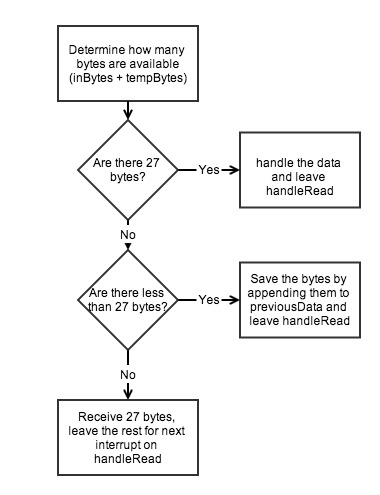
\includegraphics[keepaspectratio=true,width=0.6\linewidth]{bilder/bluetoothpc.jpg}  %skala och filnamn. 
  \end{center}
  \caption{Flödesdiagram Bluetooth mottagning} %figurtext.
  \label{fig:BTpc}
\end{figure}

\subsection{Skrivning till Bluetooth}
Skrivning till Bluetooth-enheten sker via den, i QSerialPort, inbyggda medlemsfunktionen write. I filen order.cpp finns en klass som sköter abstraktion mellan det grafiska användargränssnittet och QSerialPort. Denna har alla kommandoarrayer specificerade i sig och skickar vidare data till serialport objektet som sedan skriver denna data till Bluetooth-enheten. 

\subsection{Sensorgrafer}
Med hjälp av klassen QCustomPlot kan vi skapa grafer för plottning av sensordata från roboten. När det grafiska användargränssnittet startar sätts en timer igång. Varje gång sensor data kommer till Bluetooth-enheten tidsstämplas denna och detta används för att rita tidsberoende sensorgrafer med historik. 
Dessa grafer kan sparas ned. Då skapas en ny mapp i användarens hemkatalog kallad MapMaster och i den en textfil. Med hjälp av ett menyval, Data->Review data, öppnas ett nytt fönster med interaktiva plottar som då kan analyseras.

\subsection{Styrkommandon}
Samtliga styrkommandon är slots och funktioner utförs när knappar i det grafiska användargränssnittet trycks på eller när motsvarande knapp på tangentbordet trycks in. 
Styrkommandofunktionerna läser av hastighetsslidern och skickar sedan styrkommandot till roboten. 
\subsection{Kartan}
Kartan använder sig av Qts inbyggda klass QGraphicsScene. Objekt med dimension 10x10 skapas upp och placeras för att skapa kartan.

\section{Slutsatser}
Fler sensorer skulle kunnat förbättra kartläggning och positionering. Processorn har dock enbart 8 pinnar för ADC vilket leder till att endast 8 st sensorer med analoga utsignaler kan användas. Ett sätt att komma runt detta problem är att använda en extern mux.
Detta alternativ diskuterades i gruppen. Vi hade dock redan implementerat en fullt fungerande sensormodul, där de 8 ADC-pinnarna var fyllda, och valde därför att behålla strukturen vi hade för att unvika en tidskrävande ombyggnad från grunden.

Kortdistanssensorerna på robotens högra sida har en räckvidd på 10-80 cm. Då roboten vid reglering kan vara närmare väggen än 10 cm kan detta bli ett problem. Ett sätt att lösa problemet på är att byta sensorerna till sensorer med räckvidden 4-30 cm, 
GP2D120 som går att läsa om på Vanheden\footnote{\url{https://docs.isy.liu.se/twiki/pub/VanHeden/DataSheets/gp2d120.pdf}}. Ett byte av sensorer skulle dock innebära större begränsningar vid kartläggning.
Sensorerna var först placerade längst ut på robotens högra sida och genom att flytta dem längre in på roboten lyckades vi öka marginalen för regleringen. Vi valde därför att inte byta ut sensorerna.

Busskommunikationen fungerade ej perfekt och skulle ha kunnat förbättrats. En bufferstruktur med flertalet pekare skulle ha kunnat nyttjas. Dessutom skulle en struktur där master frågar slave-enheterna med jämna mellanrum om data istället för avbrott från slave-enheterna ha kunnat hjälpt implementeringens stabilitet.
\newpage
\section*{Referenser}
\addcontentsline{toc}{section}{Referenser}



% ----------------------------- Appendix -----------------------------------------
% --------------------------------------------------------------------------------

\newpage
\appendix
\pagestyle{empty}
\newgeometry{left=2cm,right=2cm,bottom=2cm,top=2cm}
\section*{Appendix A - Kopplingsscheman}
\addcontentsline{toc}{section}{Appendix A - Kopplingsscheman}
\subsection*{Kopplingsschema för kommunikationsmodul}

\begin{figure}[ht] %Placera här om det finns plats, annars så snart som möjligt, på toppen av en sida.
  \begin{center}
  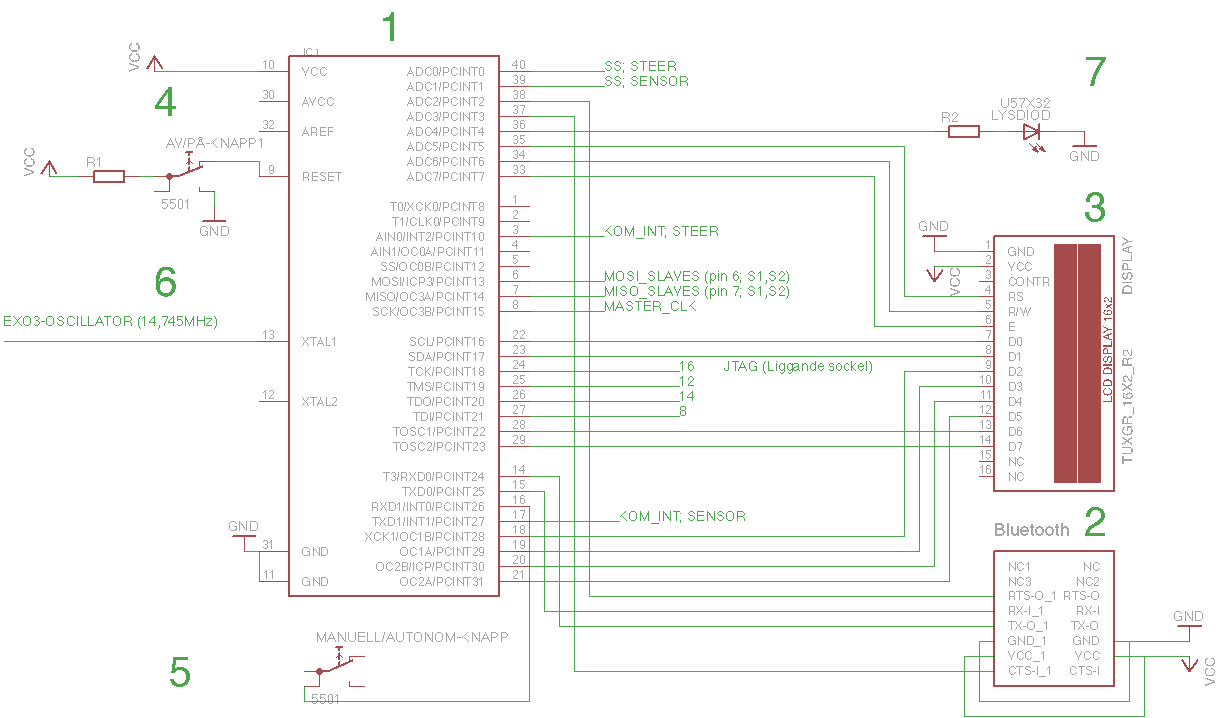
\includegraphics[keepaspectratio=true,width=\linewidth]{bilder/Kom_uptodate.png}  %skala och filnamn. 
  \end{center}
  \caption{Kopplingsschema kommunikationsmodul} %figurtext.
  \label{fig:kopplingkom} %glöm inte att uppdatera era labels
\end{figure}
 \clearpage %flushes picture cache to place now
 

\subsection*{Kopplingsschema för styrmodul}

\begin{figure}[ht] %Placera här om det finns plats, annars så snart som möjligt, på toppen av en sida.
  \begin{center}
  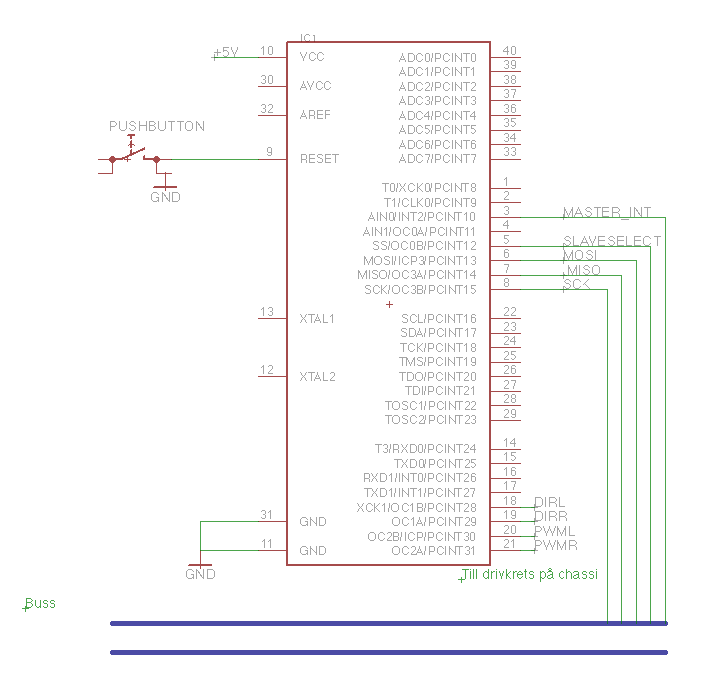
\includegraphics[keepaspectratio=true,width=\linewidth]{bilder/kopplingsschema_styrmodul.png}  %skala och filnamn. 
  \end{center}
  \caption{Kopplingsschema styrmodul} %figurtext.
  \label{fig:kopplingstyr} %glöm inte att uppdatera era labels
\end{figure}
 \clearpage %flushes picture cache to place now
 

\subsection*{Kopplingsschema för sensormodull}

\begin{figure}[ht] %Placera här om det finns plats, annars så snart som möjligt, på toppen av en sida.
  \begin{center}
  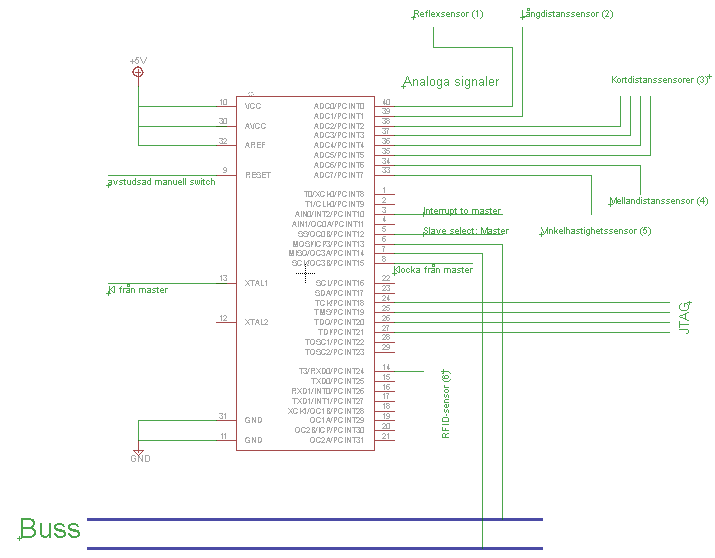
\includegraphics[keepaspectratio=true,width=\linewidth]{bilder/sensormodulkoppling.png}  %skala och filnamn. 
  \end{center}
  \caption{Kopplingsschema sensormodul} %figurtext.
  \label{fig:kopplingsensor} %glöm inte att uppdatera era labels
\end{figure}
 \clearpage %flushes picture cache to place now
 

\newpage
\section*{Appendix B - Flödesscheman}
\addcontentsline{toc}{section}{Appendix B - Flödesscheman}

\begin{figure}[htp] %Placera här om det finns plats, annars så snart som möjligt, på toppen av en sida.
  \begin{center}
  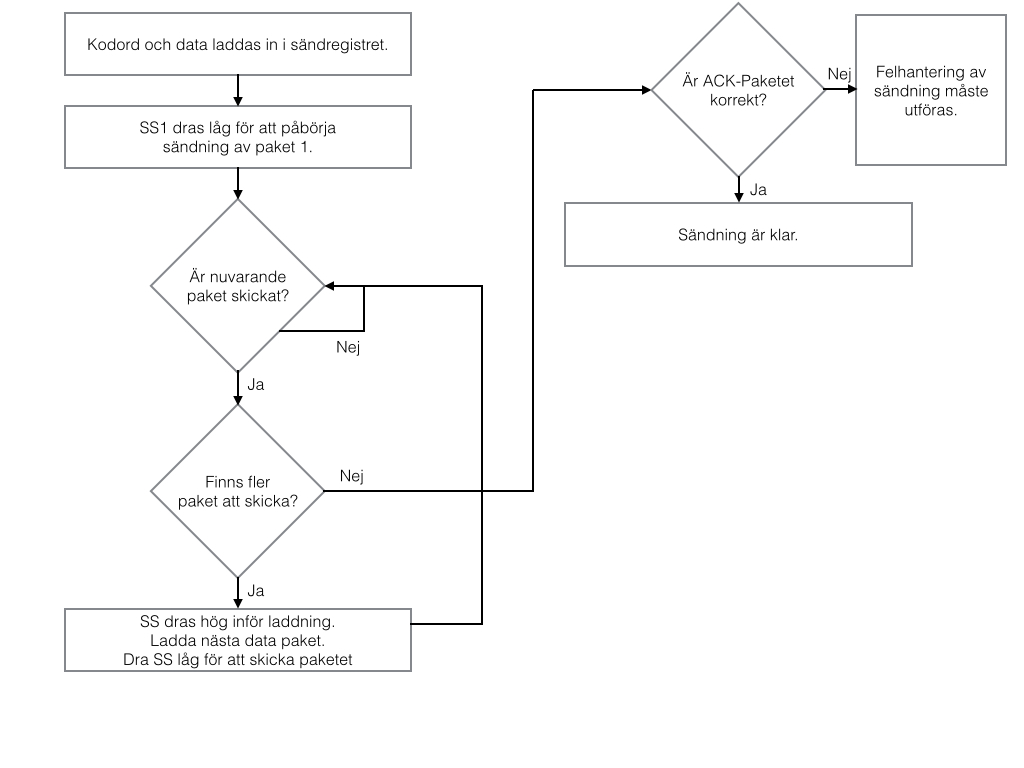
\includegraphics[keepaspectratio=true,width=\linewidth]{bilder/SPIbild002.jpg}  %skala och filnamn. 
  \end{center}
  \caption{Flödesdiagram för Fall 1.} %figurtext.
  \label{fig:case1flow}
\end{figure}

\begin{figure}[htp] %Placera här om det finns plats, annars så snart som möjligt, på toppen av en sida.
  \begin{center}
  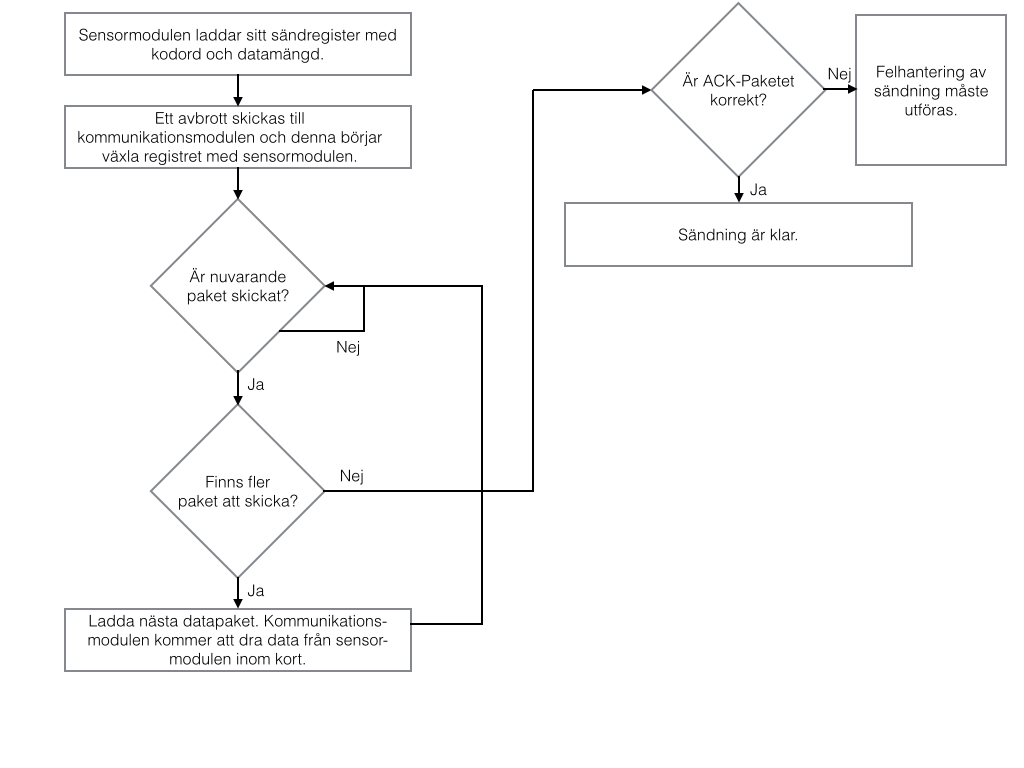
\includegraphics[keepaspectratio=true,width=\linewidth]{bilder/SPIbild003.jpg}  %skala och filnamn. 
  \end{center}
  \caption{Flödesdiagram för Fall 2.} %figurtext.
  \label{fig:case2flow}
\end{figure}
\begin{figure}[htp] %Placera här om det finns plats, annars så snart som möjligt, på toppen av en sida.
  \begin{center}
  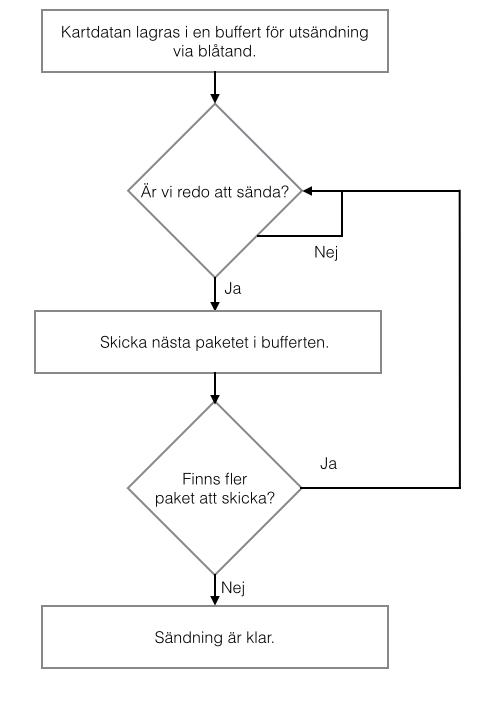
\includegraphics[keepaspectratio=true,width=0.9\linewidth]{bilder/SPIbild004.jpg}  %skala och filnamn. 
  \end{center}
  \caption{Flödesdiagram för Fall 3.} %figurtext.
  \label{fig:case3flow}
\end{figure}
\begin{figure}[htp] %Placera här om det finns plats, annars så snart som möjligt, på toppen av en sida.
  \begin{center}
  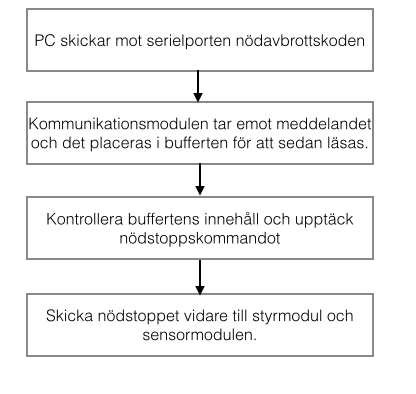
\includegraphics[keepaspectratio=true,width=0.5\linewidth]{bilder/SPIbild005.jpg}  %skala och filnamn. 
  \end{center}
  \caption{Flödesdiagram för Fall 4.} %figurtext.
  \label{fig:case4flow}
\end{figure}
\clearpage %flushes picture cache to place now
\newpage

\section*{Appendix C - Kommandon}
\addcontentsline{toc}{section}{Appendix C - Kommandon}


\begin{tabular}{| p{4cm} | p{2.5cm} | p{2.5cm} | p{2.5cm} | p{3.7cm} |}
	\hline
	\textbf{Beskrivning} & \textbf{Datalängd} & \textbf{Kommando} & \textbf{Argument} & \textbf{Data} \\ \hline
	Rotera vänster & 3 & r & 0 & 1 byte, speed \\\hline
	Rotera höger & 3 & r & 1 & 1 byte, speed \\\hline
	Halt & 3 & h & 0 & - \\\hline
	Framåt & 3 & f & 0 & 1 byte, speed \\\hline
	Bakåt & 3 & b & 0 & 1 byte, speed \\\hline
	Fetch Map & 1 & F & - & -\\\hline
	Gyro kalibrering & 2 & g & 0 & - \\\hline
	Aktivera gyro & 2 & g & 1 & - \\\hline
	Deaktivera gyro & 2 & g & 2 & - \\\hline

	Gyro 90 grader & 1 & G & - & - \\\hline
	RFID detekterad & 1 & R & - & - \\\hline
	Aktivera RFID & 1 & r & - & - \\\hline
	Kartkolumn & 19 & M & Kolumn nr& Kartkolumn\\\hline
	Bekräftar kartkolumn & 2 & m & Kolumn nr & - \\\hline
	Manuellt läge & 1 & a & - & - \\\hline
	Autonomt läge & 1 & q & - & - \\\hline
	Gyro medurskonstant & 5 & k & 0 & 3 byte,\newline [100tal 10tal 1tal]\\\hline
	Gyro moturskonstant & 5 & k & 1 & 3 byte,\newline [100tal 10tal 1tal]\\\hline
	Sensordata 0-9 & 26 & S & A & 24 bytes sensordata,\newline 8x[100tal 10tal 1tal]\\\hline
	
\end{tabular}

\end{document}>>>>>>> External Changes
